\documentclass[tikz,border=8pt]{standalone}
% Shared look for every TikZ diagram. Load with % Shared look for every TikZ diagram. Load with % Shared look for every TikZ diagram. Load with \input{../../tools/tikz-style.tex}
\usepackage[T1]{fontenc}
\usepackage{lmodern}
\renewcommand{\sfdefault}{lmr}  % diagrams use the same serif as the text
\usetikzlibrary{arrows.meta, positioning, shapes.geometric, calc, fit, backgrounds}
\definecolor{cblue}{HTML}{4C78A8}
\definecolor{corange}{HTML}{F58518}
\definecolor{cgreen}{HTML}{54A24B}
\definecolor{cred}{HTML}{E45756}
\definecolor{cpurple}{HTML}{B279A2}
\definecolor{cgrey}{HTML}{6B6B6B}
\tikzset{
  every picture/.style={font=\sffamily, line width=1.2pt},
  box/.style={draw=#1, fill=#1!12, rounded corners=4pt, align=center, inner sep=7pt, minimum height=1.1cm},
  box/.default=cgrey,
  arrow/.style={-{Stealth[length=3mm]}, draw=cgrey, line width=1.4pt},
  title/.style={font=\sffamily\bfseries\Large},
  note/.style={font=\sffamily\small, text=cgrey, align=center},
}
\AtBeginDocument{\hyphenpenalty=10000 \exhyphenpenalty=10000}

\usepackage[T1]{fontenc}
\usepackage{lmodern}
\renewcommand{\sfdefault}{lmr}  % diagrams use the same serif as the text
\usetikzlibrary{arrows.meta, positioning, shapes.geometric, calc, fit, backgrounds}
\definecolor{cblue}{HTML}{4C78A8}
\definecolor{corange}{HTML}{F58518}
\definecolor{cgreen}{HTML}{54A24B}
\definecolor{cred}{HTML}{E45756}
\definecolor{cpurple}{HTML}{B279A2}
\definecolor{cgrey}{HTML}{6B6B6B}
\tikzset{
  every picture/.style={font=\sffamily, line width=1.2pt},
  box/.style={draw=#1, fill=#1!12, rounded corners=4pt, align=center, inner sep=7pt, minimum height=1.1cm},
  box/.default=cgrey,
  arrow/.style={-{Stealth[length=3mm]}, draw=cgrey, line width=1.4pt},
  title/.style={font=\sffamily\bfseries\Large},
  note/.style={font=\sffamily\small, text=cgrey, align=center},
}
\AtBeginDocument{\hyphenpenalty=10000 \exhyphenpenalty=10000}

\usepackage[T1]{fontenc}
\usepackage{lmodern}
\renewcommand{\sfdefault}{lmr}  % diagrams use the same serif as the text
\usetikzlibrary{arrows.meta, positioning, shapes.geometric, calc, fit, backgrounds}
\definecolor{cblue}{HTML}{4C78A8}
\definecolor{corange}{HTML}{F58518}
\definecolor{cgreen}{HTML}{54A24B}
\definecolor{cred}{HTML}{E45756}
\definecolor{cpurple}{HTML}{B279A2}
\definecolor{cgrey}{HTML}{6B6B6B}
\tikzset{
  every picture/.style={font=\sffamily, line width=1.2pt},
  box/.style={draw=#1, fill=#1!12, rounded corners=4pt, align=center, inner sep=7pt, minimum height=1.1cm},
  box/.default=cgrey,
  arrow/.style={-{Stealth[length=3mm]}, draw=cgrey, line width=1.4pt},
  title/.style={font=\sffamily\bfseries\Large},
  note/.style={font=\sffamily\small, text=cgrey, align=center},
}
\AtBeginDocument{\hyphenpenalty=10000 \exhyphenpenalty=10000}

\begin{document}
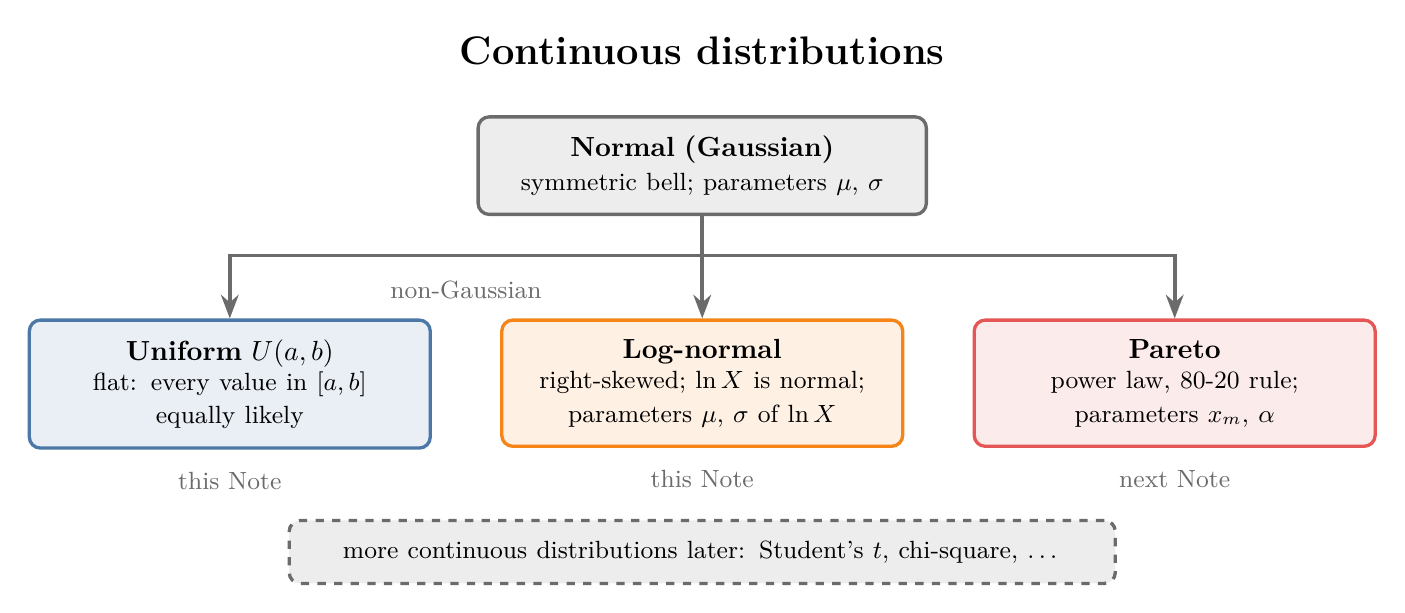
\begin{tikzpicture}[node distance=0.7cm and 0.5cm]
  \node[title] (t) {Continuous distributions};
  \node[box=cgrey, below=0.5cm of t, text width=5.2cm] (normal) {\textbf{Normal (Gaussian)}\\ \small symmetric bell; parameters $\mu$, $\sigma$};
  \node[box=cblue, below=1.3cm of normal, xshift=-6cm, text width=4.6cm] (uni) {\textbf{Uniform} $U(a, b)$\\ \small flat: every value in $[a, b]$\\ equally likely};
  \node[box=corange, below=1.3cm of normal, text width=4.6cm] (logn) {\textbf{Log-normal}\\ \small right-skewed; $\ln X$ is normal;\\ parameters $\mu$, $\sigma$ of $\ln X$};
  \node[box=cred, below=1.3cm of normal, xshift=6cm, text width=4.6cm] (par) {\textbf{Pareto}\\ \small power law, 80-20 rule;\\ parameters $x_m$, $\alpha$};
  \node[note, above=0.12cm of logn, xshift=-3cm] {non-Gaussian};
  \draw[arrow] (normal.south) -- ++(0,-0.5) -| (uni.north);
  \draw[arrow] (normal.south) -- (logn.north);
  \draw[arrow] (normal.south) -- ++(0,-0.5) -| (par.north);
  \node[note, below=0.15cm of uni] {this Note};
  \node[note, below=0.15cm of logn] {this Note};
  \node[note, below=0.15cm of par] {next Note};
  \node[box=cgrey, below=0.9cm of logn, text width=10cm, minimum height=0.8cm, dashed] (later) {\small more continuous distributions later: Student's $t$, chi-square, \dots};
\end{tikzpicture}
\end{document}
